\documentclass[11pt]{article}
\usepackage{./EllioStyle}
\usepackage{listings}
\usepackage{pdfpages}

\definecolor{codegreen}{rgb}{0,0.6,0}
\definecolor{codegray}{rgb}{0.5,0.5,0.5}
\definecolor{codepurple}{rgb}{0.58,0,0.82}
\definecolor{backcolour}{rgb}{0.95,0.95,0.92}

\title{Homework 2}
\author{Elliott Pryor}
\date{23 September 2021}

\rhead{Homework 2}

\begin{document}
\maketitle

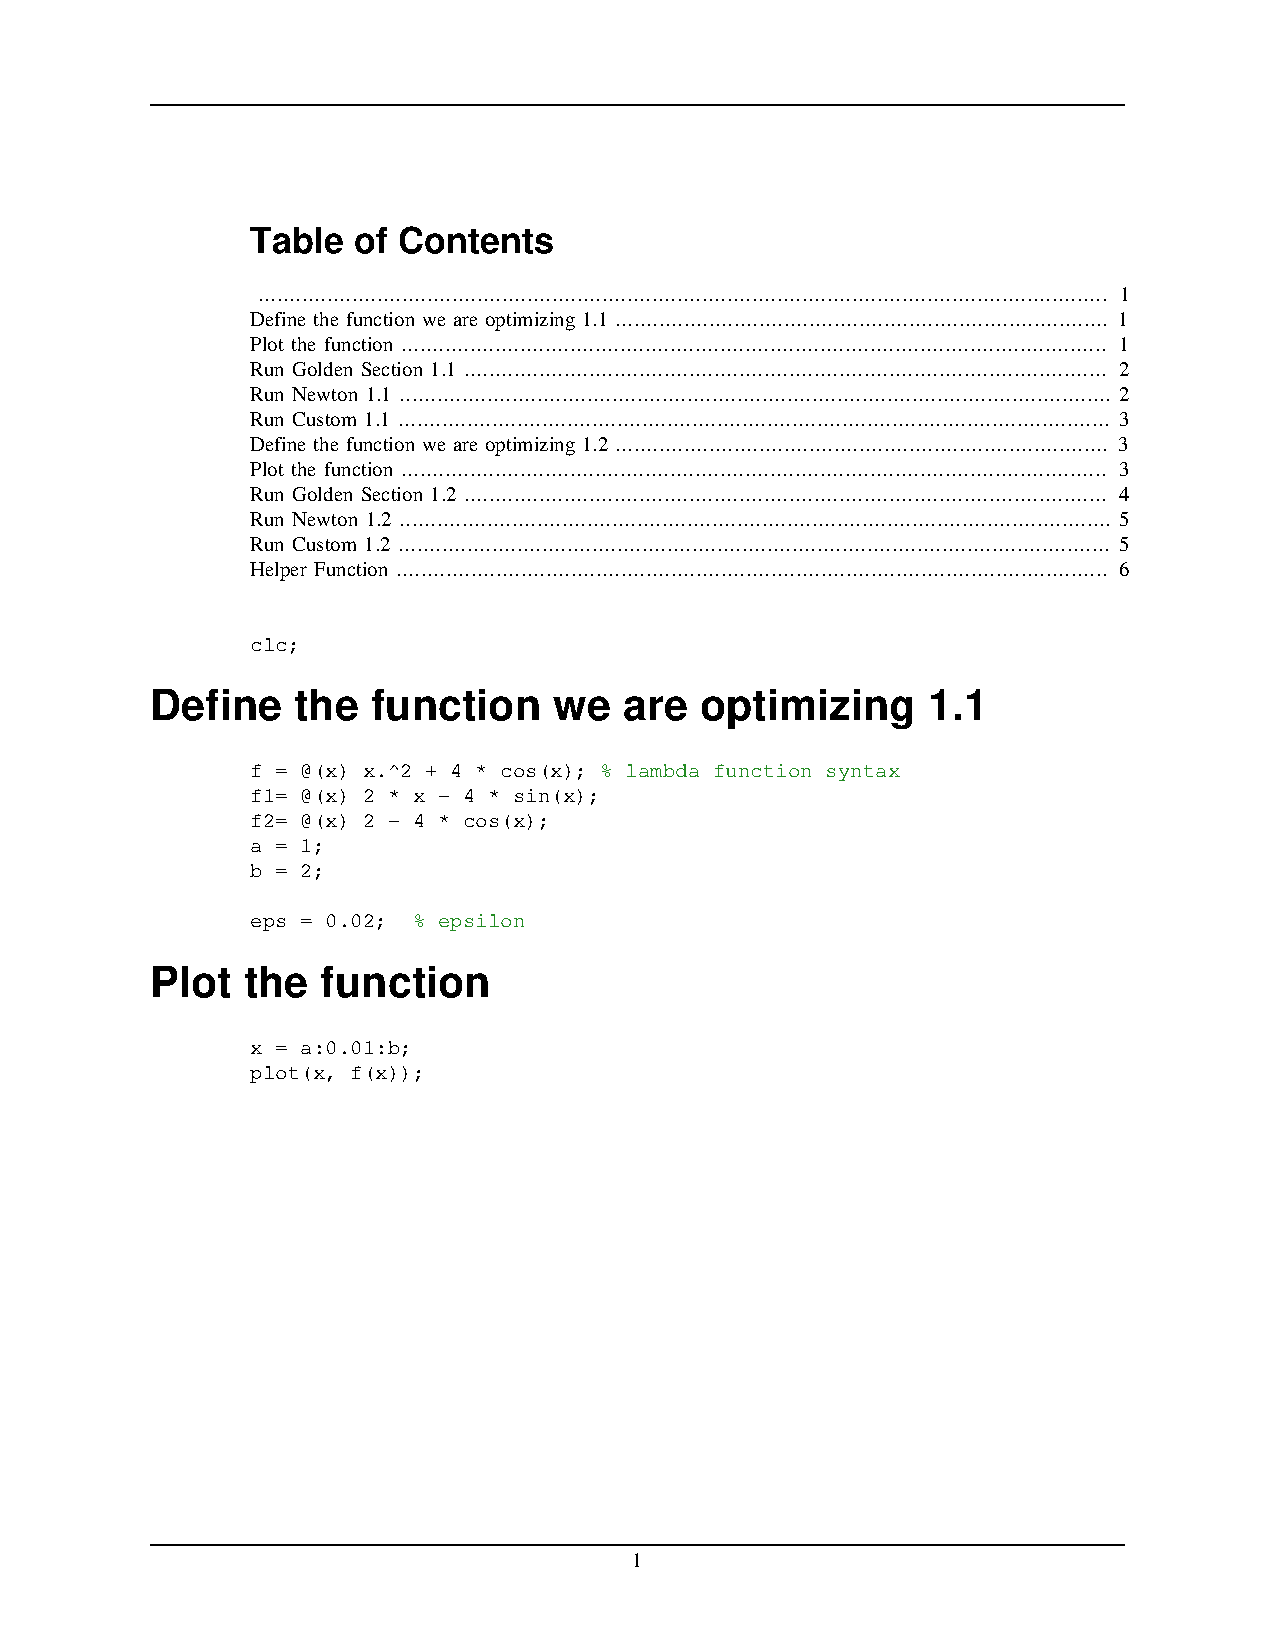
\includepdf[pages=-]{golden_section.pdf}

\problem{2}
Derive a one-dimensional minimization algorithm based on quadratic fit that only requires objective function
values (but no derivatives). Specifically, derive an algorithm that computes $x_{k+1}$
based on $x_k,x_{k-1},x_{k-2}$, and $f(x_k),f(x_{k-1}),f(x_{k-2})$. 
Hint: To simplify notation, used
$\delta_{i,j} = x_{k-i} - x_{k-j}$ and $\sigma_{i,j} = (x_{k-i})^2 - (x_{k-j})^2$

Bonus: implement your algorithm as a MATLAB script and apply it to the numerical problems, above. 
Note that you will needthree points to initialize the algorithm.

\hrule

We want to solve this linear equation 

$$\begin{bmatrix}
    x_k^2 & x_k & 1 \\
    x_{k-1}^2 & x_{k-1} & 1 \\
    x_{k-2}^2 & x_{k-2} & 1
    \end{bmatrix}
    \begin{bmatrix}
        a \\
        b \\
        c
    \end{bmatrix}
    =
    \begin{bmatrix}
        f(x_k) \\
        f(x_{k-1}) \\
        f(x_{k-2})
    \end{bmatrix}
    $$

    We use cramer's rule to solve this.

$$D = \begin{vmatrix}
    x_k^2 & x_k & 1 \\
    x_{k-1}^2 & x_{k-1} & 1 \\
    x_{k-2}^2 & x_{k-2} & 1
    \end{vmatrix}
    = x_k^2 \delta_{1,2} + x_k \sigma_{2,1} + x_{k-1}x_{k-2} \delta_{1,2}
$$

$$D_a = \begin{vmatrix}
    f(x_k) & x_k & 1 \\
    f(x_{k-1}) & x_{k-1} & 1 \\
    f(x_{k-2}) & x_{k-2} & 1
    \end{vmatrix}
    = f(x_k)\delta_{1,2} + f(x_{k-1})\delta_{2,0} + f(x_{k-2})\delta_{0,1}
$$

$$
Db = f(x_{k-1}) \sigma{0,2} + f(x_{k-2}) \sigma{1,0} + f(x_k) \sigma{2, 1}
$$

$$
D_c = x_k^2(x_{k-1}f(x_{k-2})-x_{k-2}f(x_{k-1}))-x_k(x_{k-1}^2f(x_{k-2}) -x_{k-2}f(x_{k-1}))+f(x_k)(x_{k-1}^2x_{k-2}-x_{k-2}^2x_{k-1})
$$

We know for a quadratic the minimum occurs at $-b / 2a$. So we can now solve using Cramer's rule.

\begin{align*}
    x_{k+1} &= \frac{-b}{2a}\\
    &= \frac{- D_b}{D} * \frac{D}{2 * D_a} \\
    &= \frac{-D_b}{2 * D_a}\\
    &= \frac{-f(x_{k-1}) \sigma_{0,2} - f(x_{k-2}) \sigma_{1,0} - f(x_k) \sigma_{2, 1}}{2 * (f(x_k)\delta_{1,2} + f(x_{k-1})\delta_{2,0} + f(x_{k-2})\delta_{0,1})}
\end{align*}



\end{document}